\documentclass[14pt]{article}
\title{Assignment2 Report}
\author{Zepeng Chen}
\date{\today}
\usepackage{listings}
\usepackage{color}
\usepackage{graphicx}
\usepackage{subcaption}
\usepackage{gensymb}
\usepackage{geometry}
\geometry{a4paper,left=2cm,right=2cm,top=1cm,bottom=1cm}

\definecolor{dkgreen}{rgb}{0,0.6,0}
\definecolor{gray}{rgb}{0.5,0.5,0.5}
\definecolor{mauve}{rgb}{0.58,0,0.82}

\lstset{frame=tb,
	language=Matlab,
	aboveskip=3mm,
	belowskip=3mm,
	showstringspaces=false,
	columns=flexible,
	basicstyle={\small\ttfamily},
	numbers=none,
	numberstyle=\tiny\color{gray},
	keywordstyle=\color{blue},
	commentstyle=\color{dkgreen},
	stringstyle=\color{mauve},
	breaklines=true,
	breakatwhitespace=true,
	tabsize=3
}

\begin{document}
	\maketitle
	\tableofcontents
	\newcommand{\RNum}[1]{\uppercase\expandafter{\romannumeral #1\relax}}
	\section{Part \RNum{1}:code for manually add noise}
	\lstinputlisting[breaklines]{as2.m}
	\section{Part \RNum{2}:code for filters}
	\lstinputlisting[breaklines]{filters.m}
	\section{Part \RNum{3}: questions answer}
		1.~	FSmax is:23229905\\
		2.~
			\begin{figure}[hbt!]
				\centering
				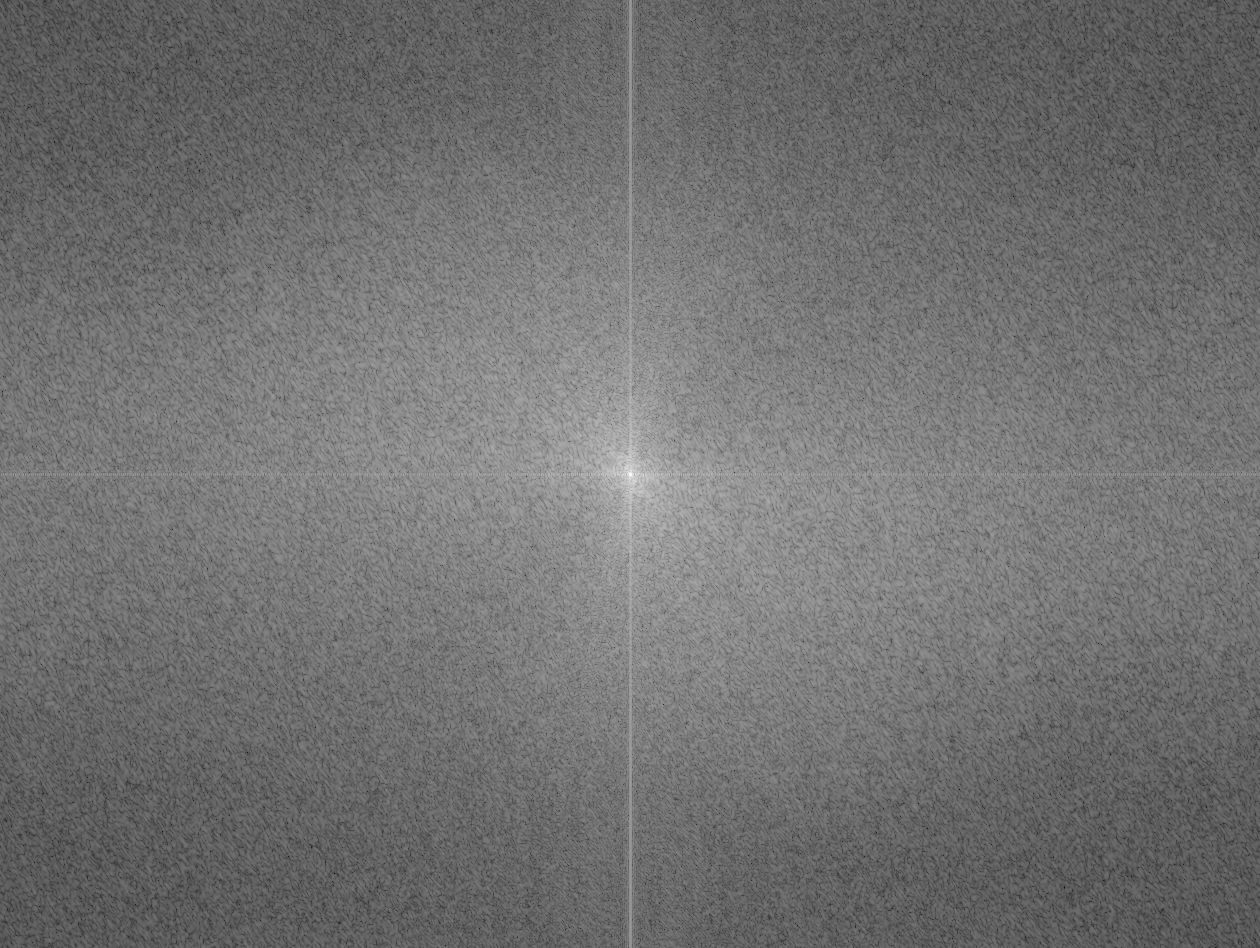
\includegraphics[width=\linewidth]{ori_spec.png}
				\caption{Original Spectrum.}
			\end{figure}
		\newpage
		3.~
			\begin{figure}[hbt!]
				\centering
				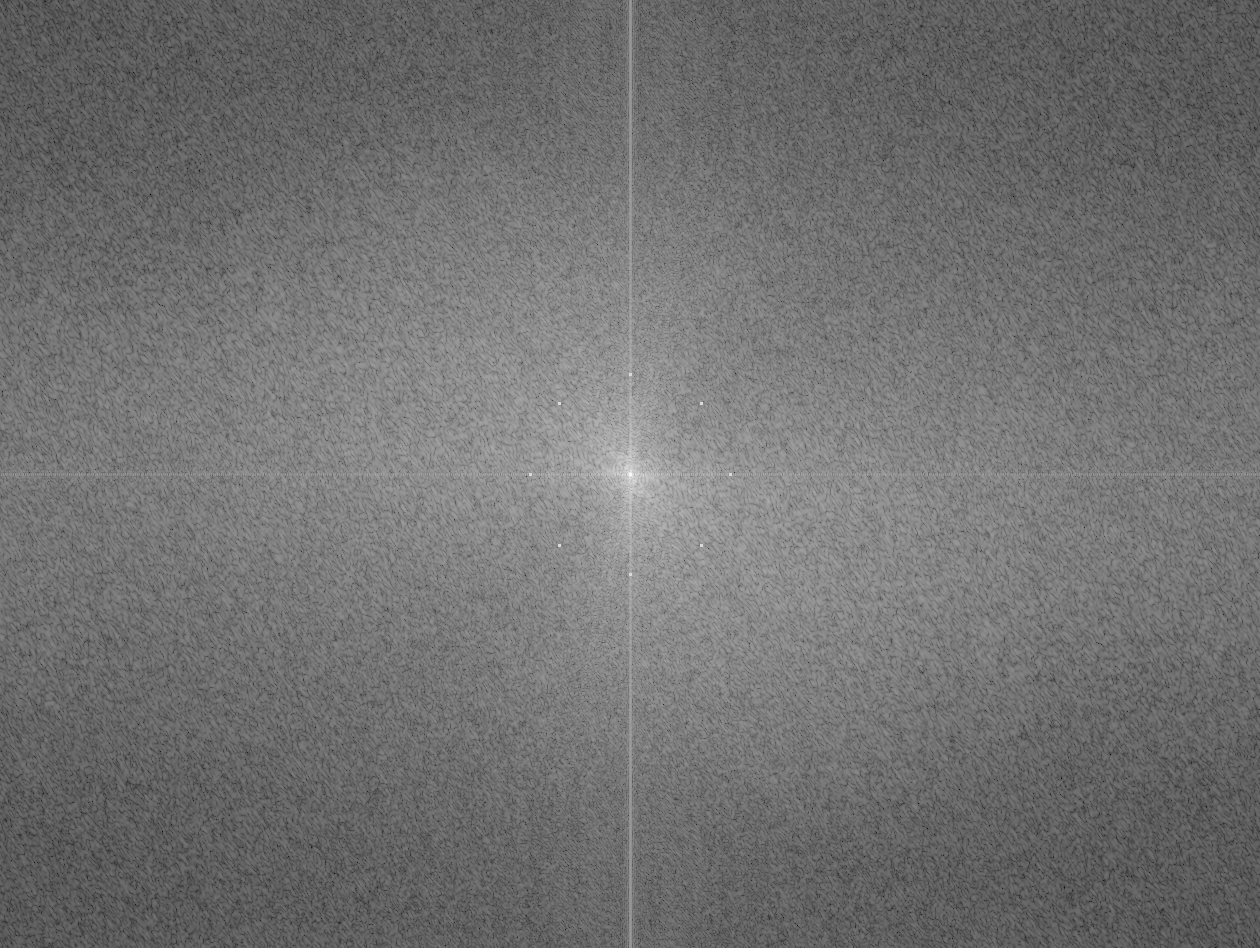
\includegraphics[width=\linewidth]{noise_added_spec.png}
				\caption{manual noise spectrum}
			\end{figure}
		\newpage
		4.~
			\begin{figure}[hbt!]
				\centering
				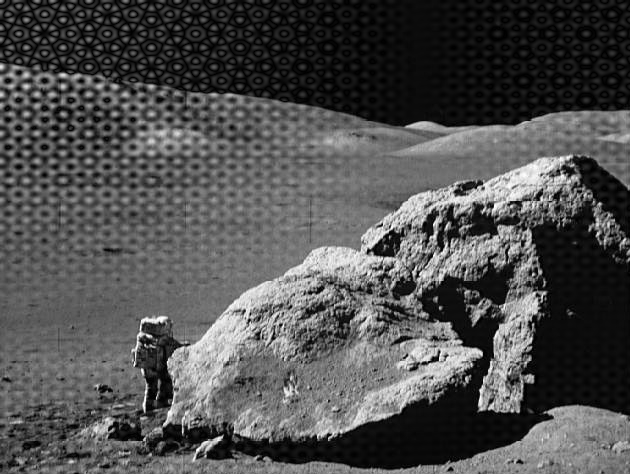
\includegraphics[width=\linewidth]{noise_added_img.png}
			\end{figure}
		We can found there are circles periodically repeating with dark and bright strip. Because we manually add eight 3x3 square in spectrum. The square function's inverse fourier transformation is sinc function. So after we ifft the noise added spectrum we get that pattern noise.\\\\
		5.~
			\begin{figure}[hbt!]
				\centering
				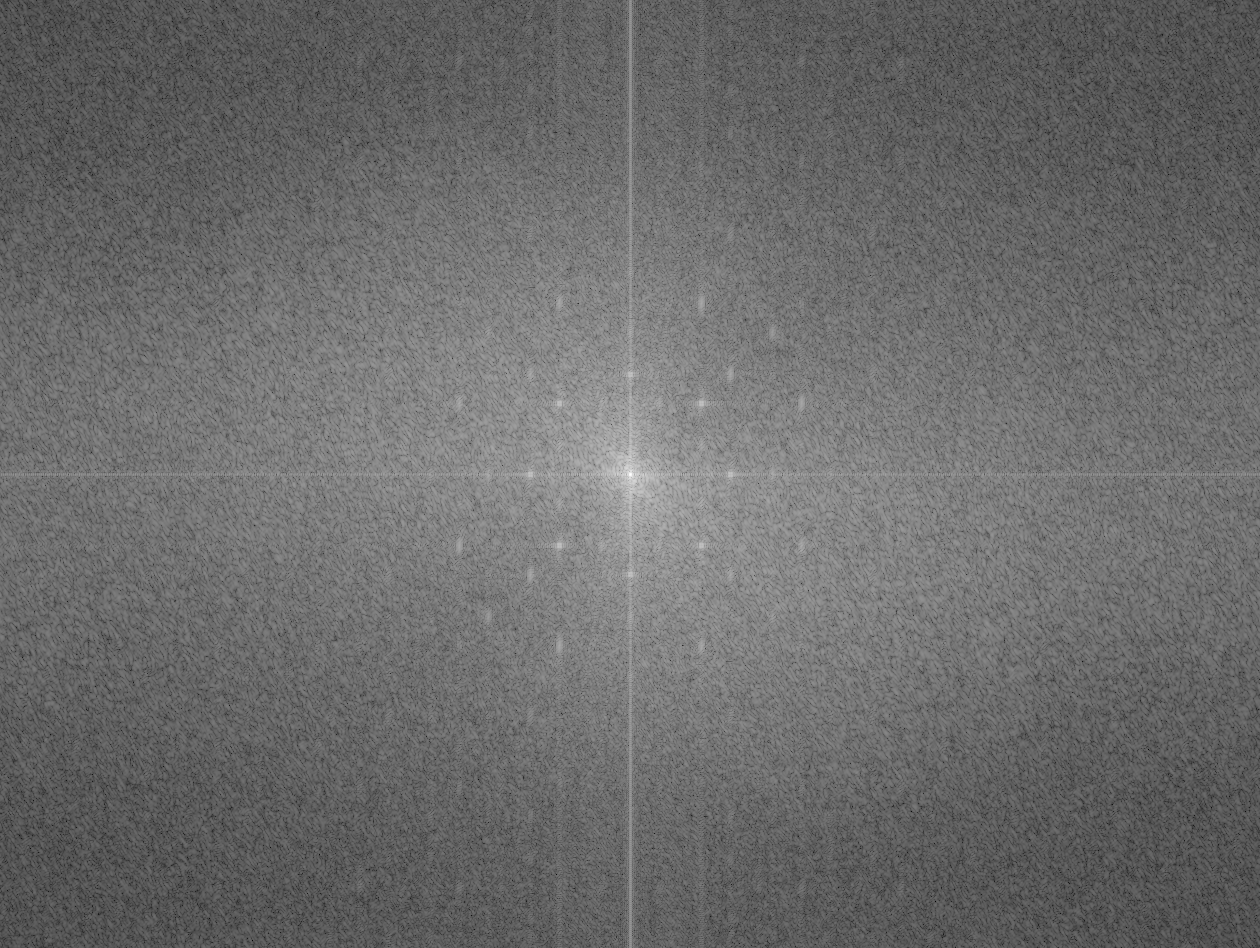
\includegraphics[width=\linewidth]{noise_spec.png}
				\caption{noise spectrum}
			\end{figure}
		From the image, we can see the spectrum transformed from the noise image does not look like what I created manually.\\\\
		\newpage
		6.~
			\begin{figure}[hbt!]
				\centering
				
					
\includegraphics[width=0.9\linewidth]{ideal.png}
					\caption{ideal filter.}
			\end{figure}
			
				\begin{figure}[hbt!]
					\centering
					
\includegraphics[width=0.9\linewidth]{btw.png}
					\caption{butterworth filter.}
				\end{figure}
				\begin{figure}[hbt!]
					\centering
					
\includegraphics[width=0.9\linewidth]{gaussian.png}
					\caption{gaussian filter.}
			\end{figure}
		\newpage
		7.~
			\begin{figure}[hbt!]
				\centering
				\begin{subfigure}[b]{0.3\linewidth}
					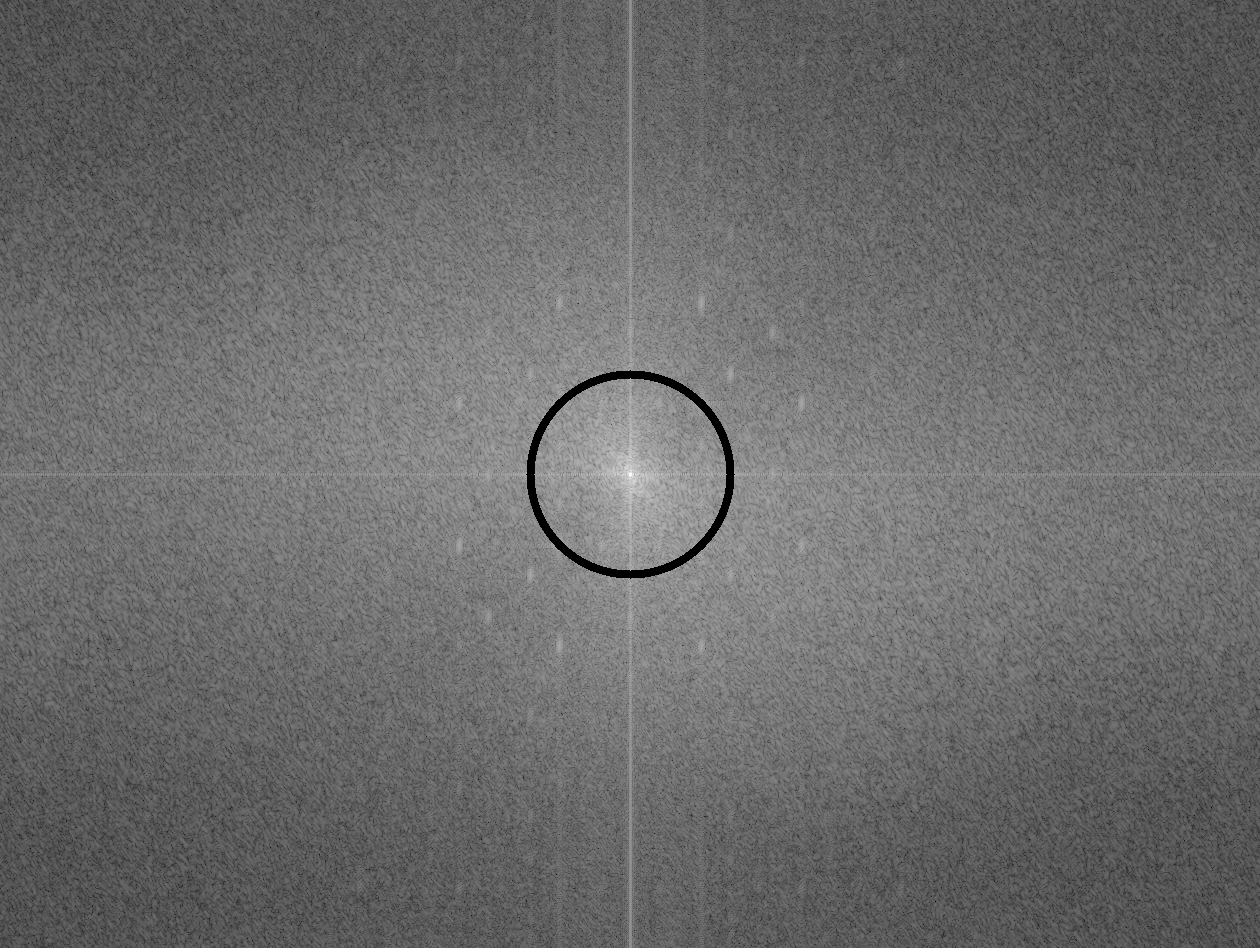
\includegraphics[width=\linewidth]{ideal_filtered_spec.png}
					\caption{ideal filtered.}
				\end{subfigure}
				\begin{subfigure}[b]{0.3\linewidth}
					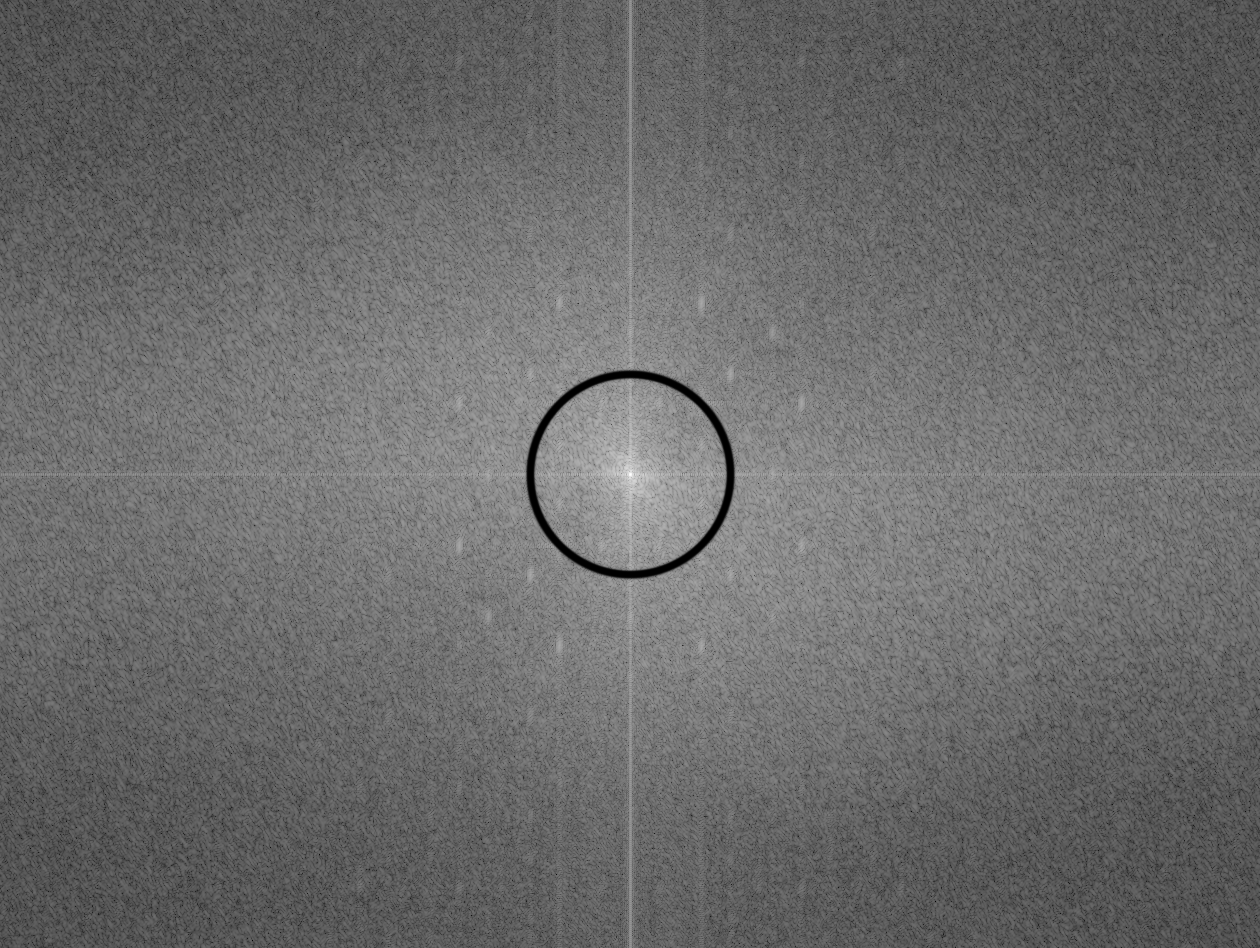
\includegraphics[width=\linewidth]{btw_filtered_spec.png}
					\caption{butterworth filtered.}
				\end{subfigure}
				\begin{subfigure}[b]{0.3\linewidth}
					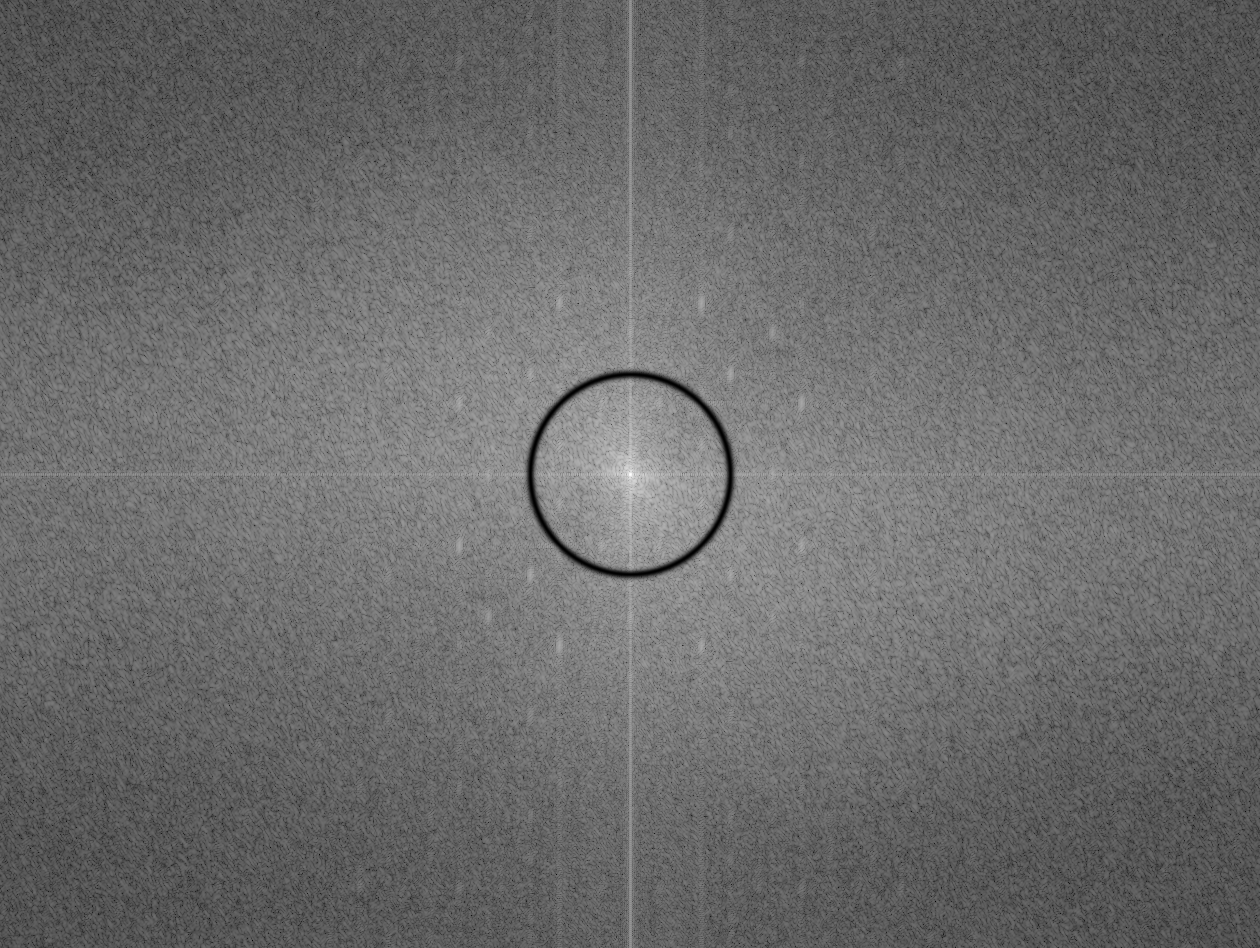
\includegraphics[width=\linewidth]{gaussian_filtered_spec.png}
					\caption{gaussian filtered.}
				\end{subfigure}
			\caption{Filters applied to the spectrum transformed back from manually added noise.}
			\label{fig:back}
			\end{figure}
		
		\begin{figure}[hbt!]
			\centering
			\begin{subfigure}[b]{0.3\linewidth}
				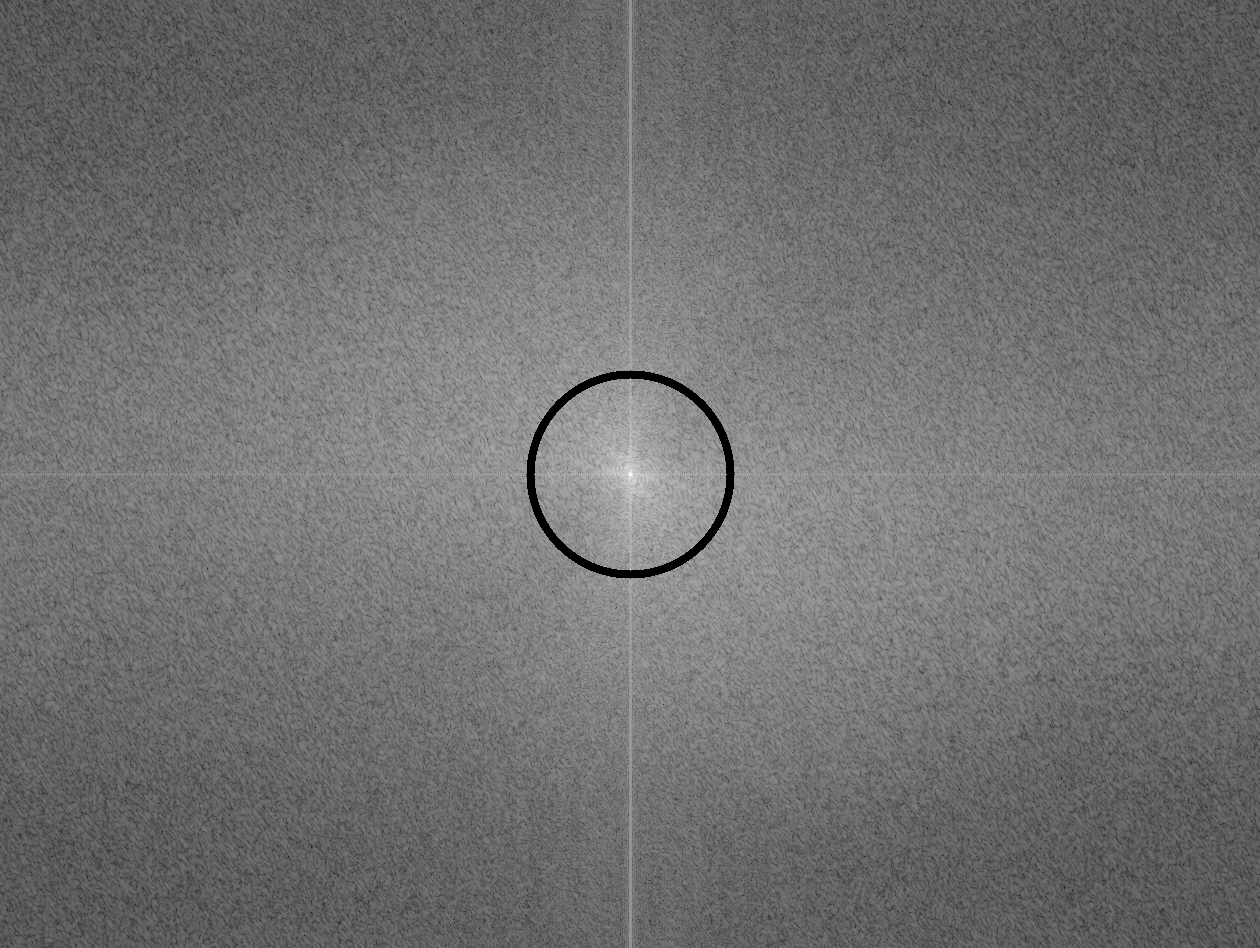
\includegraphics[width=\linewidth]{ideal_filtered_spec_man.png}
				\caption{ideal filtered.}
			\end{subfigure}
			\begin{subfigure}[b]{0.3\linewidth}
				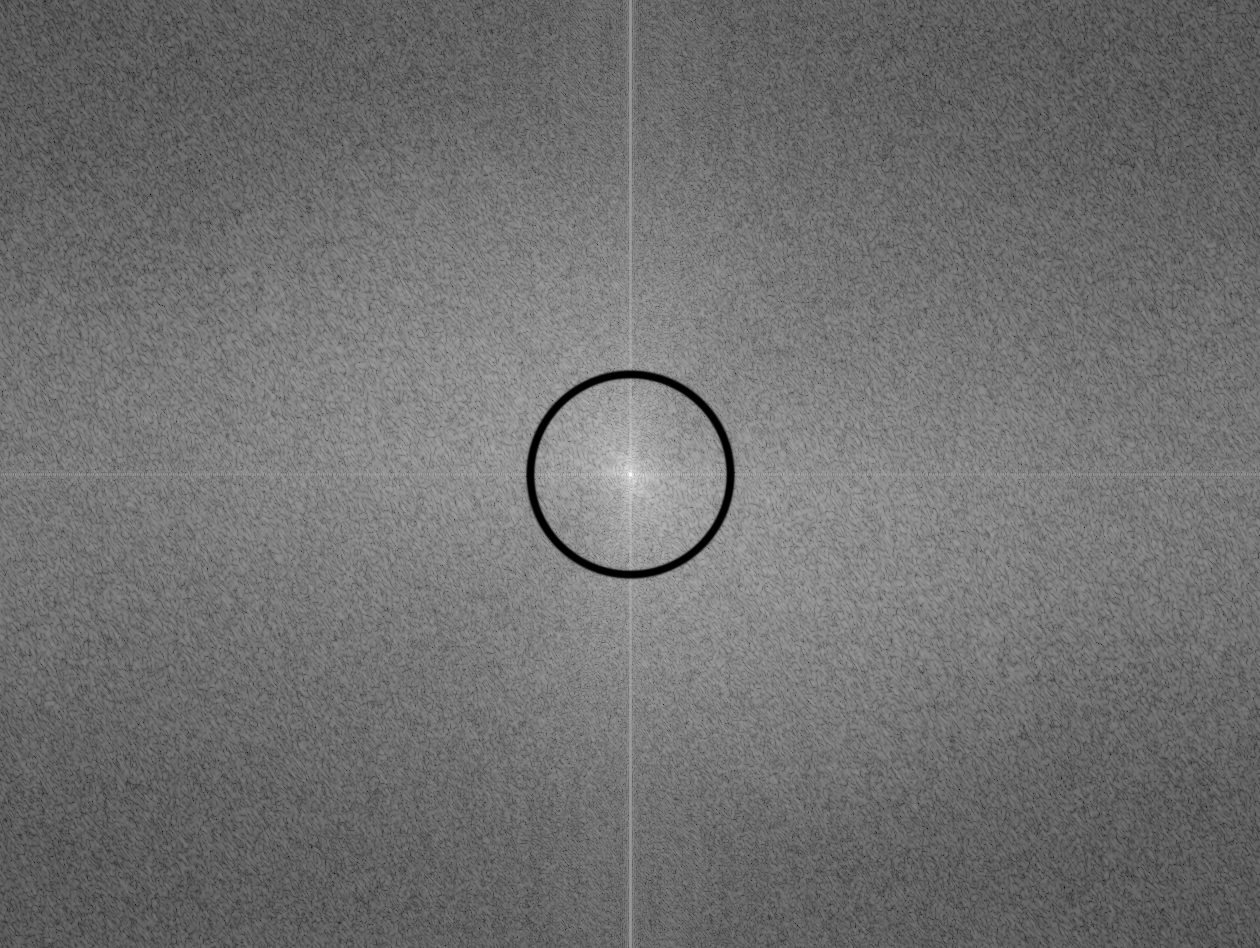
\includegraphics[width=\linewidth]{btw_filtered_spec_man.png}
				\caption{butterworth filtered.}
			\end{subfigure}
			\begin{subfigure}[b]{0.3\linewidth}
				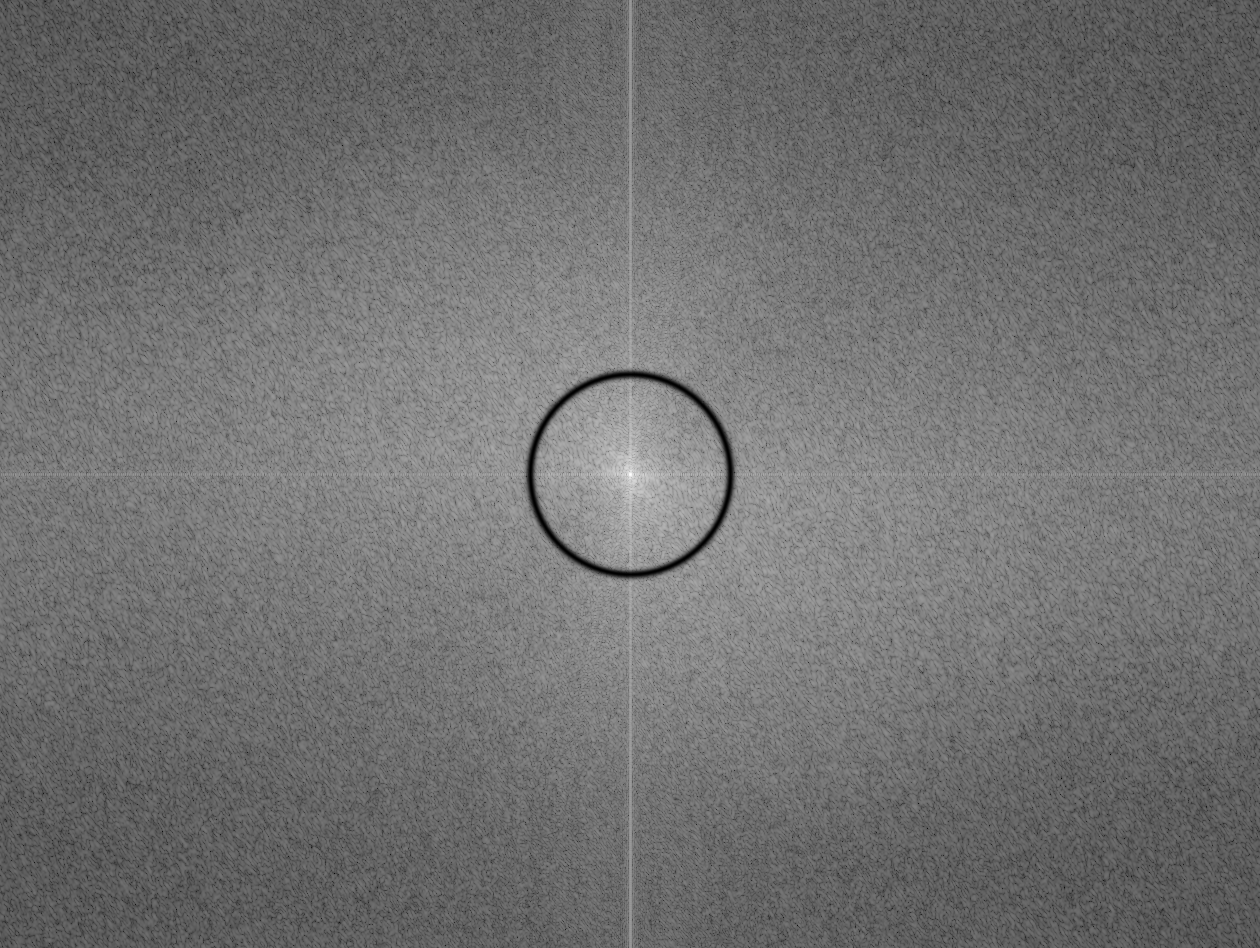
\includegraphics[width=\linewidth]{gaussian_filtered_spec_man.png}
				\caption{gaussian filtered.}
			\end{subfigure}
			\caption{Filters applied to the manually added noise spectrum directly.}
			\label{fig:direct}
		\end{figure}
		\newpage
	8.~
		\begin{figure}[hbt!]
			\centering
			\begin{subfigure}[b]{0.3\linewidth}
				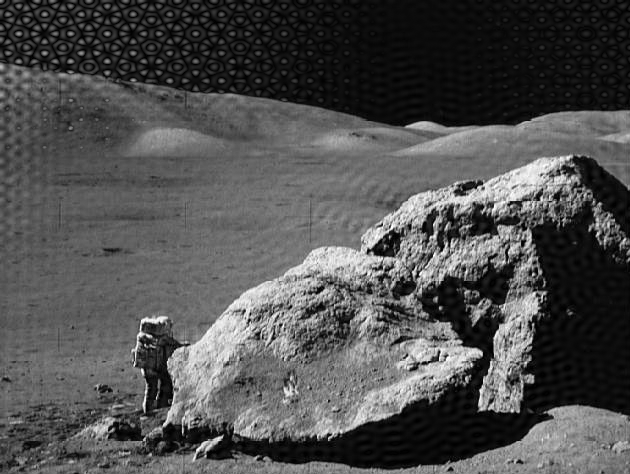
\includegraphics[width=\linewidth]{ideal_image.png}
				\caption{ideal filtered image.}
			\end{subfigure}
			\begin{subfigure}[b]{0.3\linewidth}
				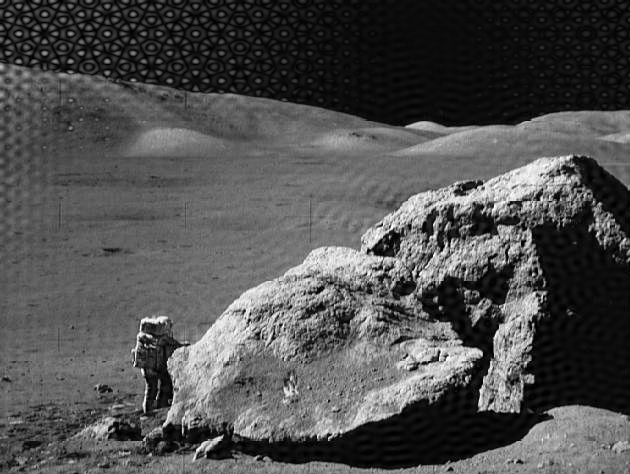
\includegraphics[width=\linewidth]{btw_image.png}
				\caption{btw filtered image.}
			\end{subfigure}
			\begin{subfigure}[b]{0.3\linewidth}
				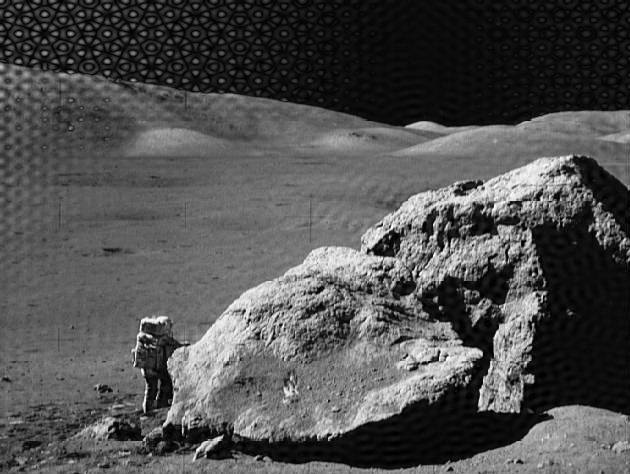
\includegraphics[width=\linewidth]{gaussian_image.png}
				\caption{gaussian filtered image.}
			\end{subfigure}
	\caption{The resultant filtered images correspond to Figure \ref{fig:back}}
		\end{figure}
	
	\begin{figure}[hbt!]
		\centering
		\begin{subfigure}[b]{0.3\linewidth}
			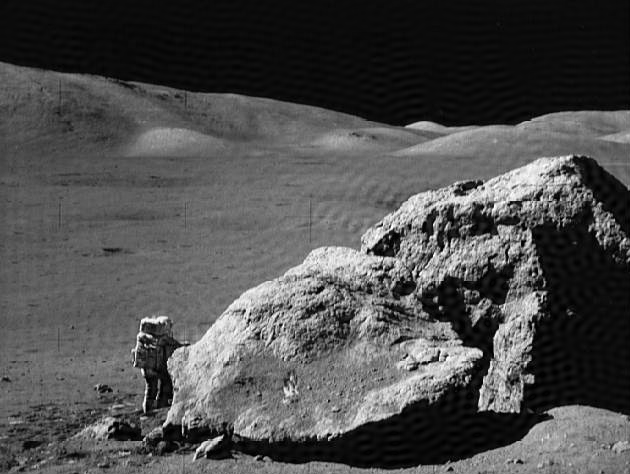
\includegraphics[width=\linewidth]{ideal_image_man.png}
			\caption{ideal filtered image.}
		\end{subfigure}
		\begin{subfigure}[b]{0.3\linewidth}
			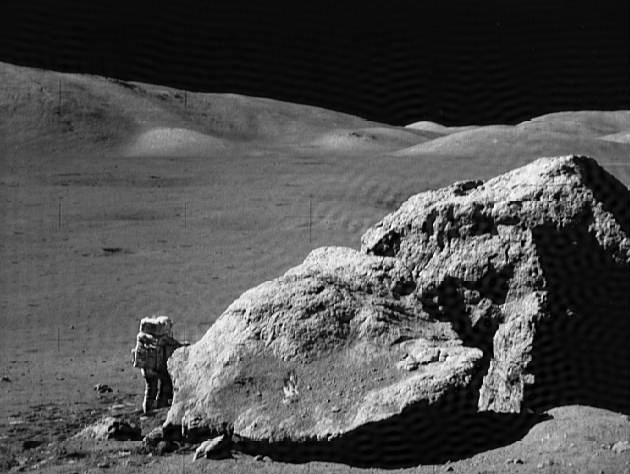
\includegraphics[width=\linewidth]{btw_image_man.png}
			\caption{btw filtered image.}
		\end{subfigure}
		\begin{subfigure}[b]{0.3\linewidth}
			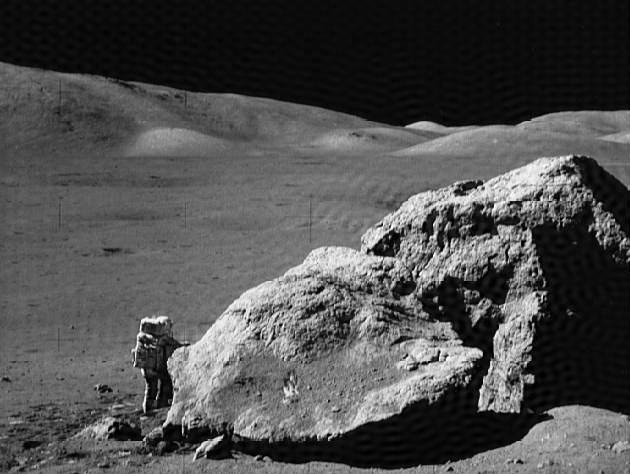
\includegraphics[width=\linewidth]{gaussian_image_man.png}
			\caption{gaussian filtered image.}
		\end{subfigure}
		\caption{The resultant filtered images correspond to Figure \ref{fig:direct}}
	\end{figure}
		Compare the above images with (a) the noise added image, the filter does remove most noise noticeably. While compare with (b) the original image, there are some noise still existing in the top-left corner. If we apply the filter to manually added noise spectrum directly, we can remove it properly for the filters can fully cover the eight dots. We still can find some noise like ripples because when we apply the filters, not only were the noise frequency dots removed, but also the useful frequency.
		\newpage
	9.~
	\begin{figure}[hbt!]
		\centering
		\begin{subfigure}[b]{0.3\linewidth}
			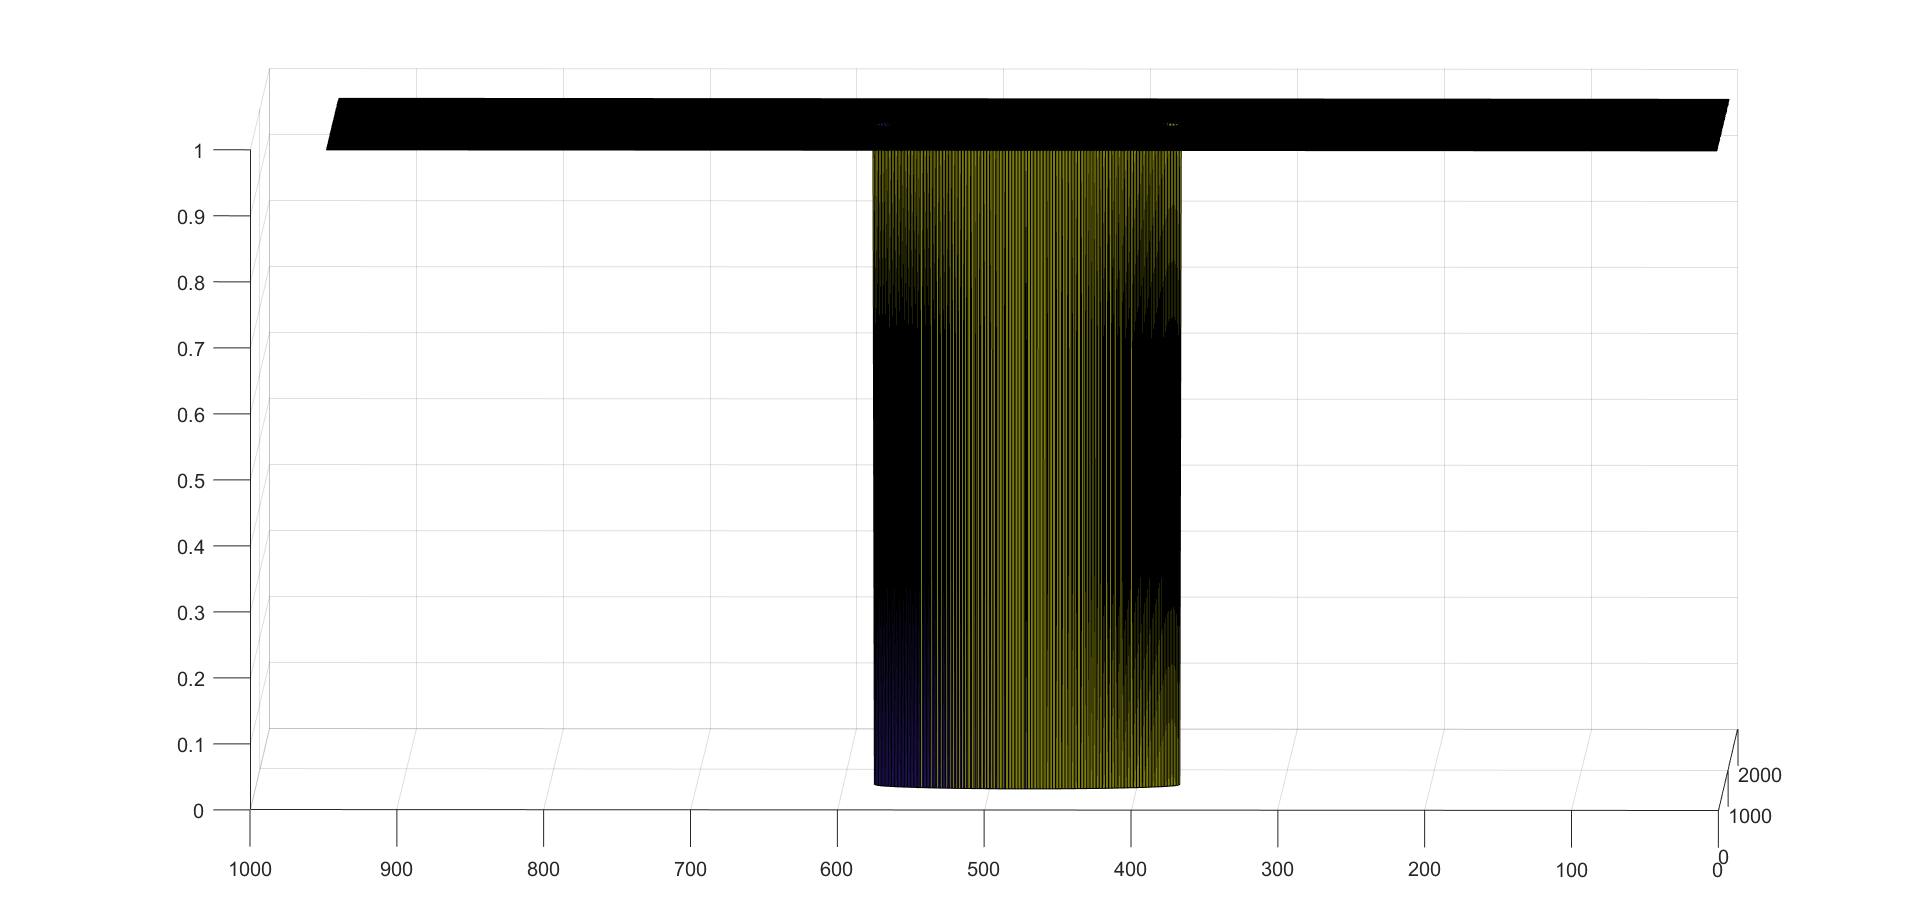
\includegraphics[width=\linewidth]{ideal3d.png}
			\caption{ideal.}
		\end{subfigure}
		\begin{subfigure}[b]{0.3\linewidth}
			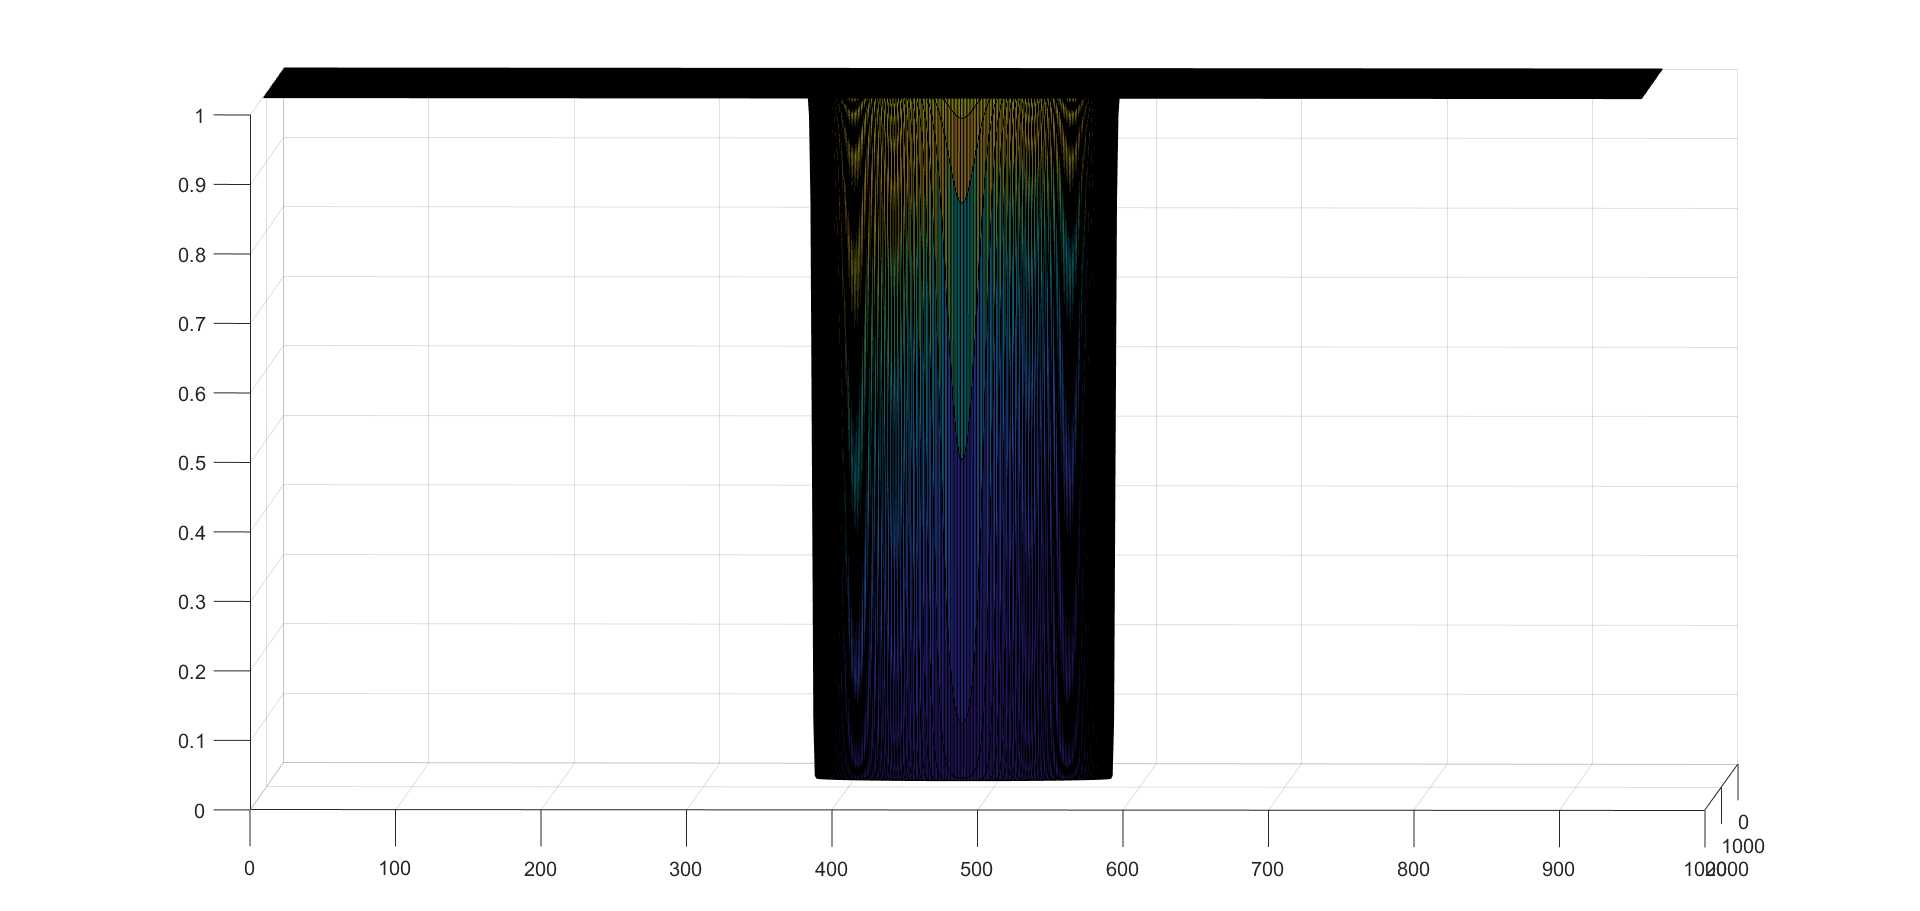
\includegraphics[width=\linewidth]{btw3d.png}
			\caption{butterworth.}
		\end{subfigure}
		\begin{subfigure}[b]{0.3\linewidth}
			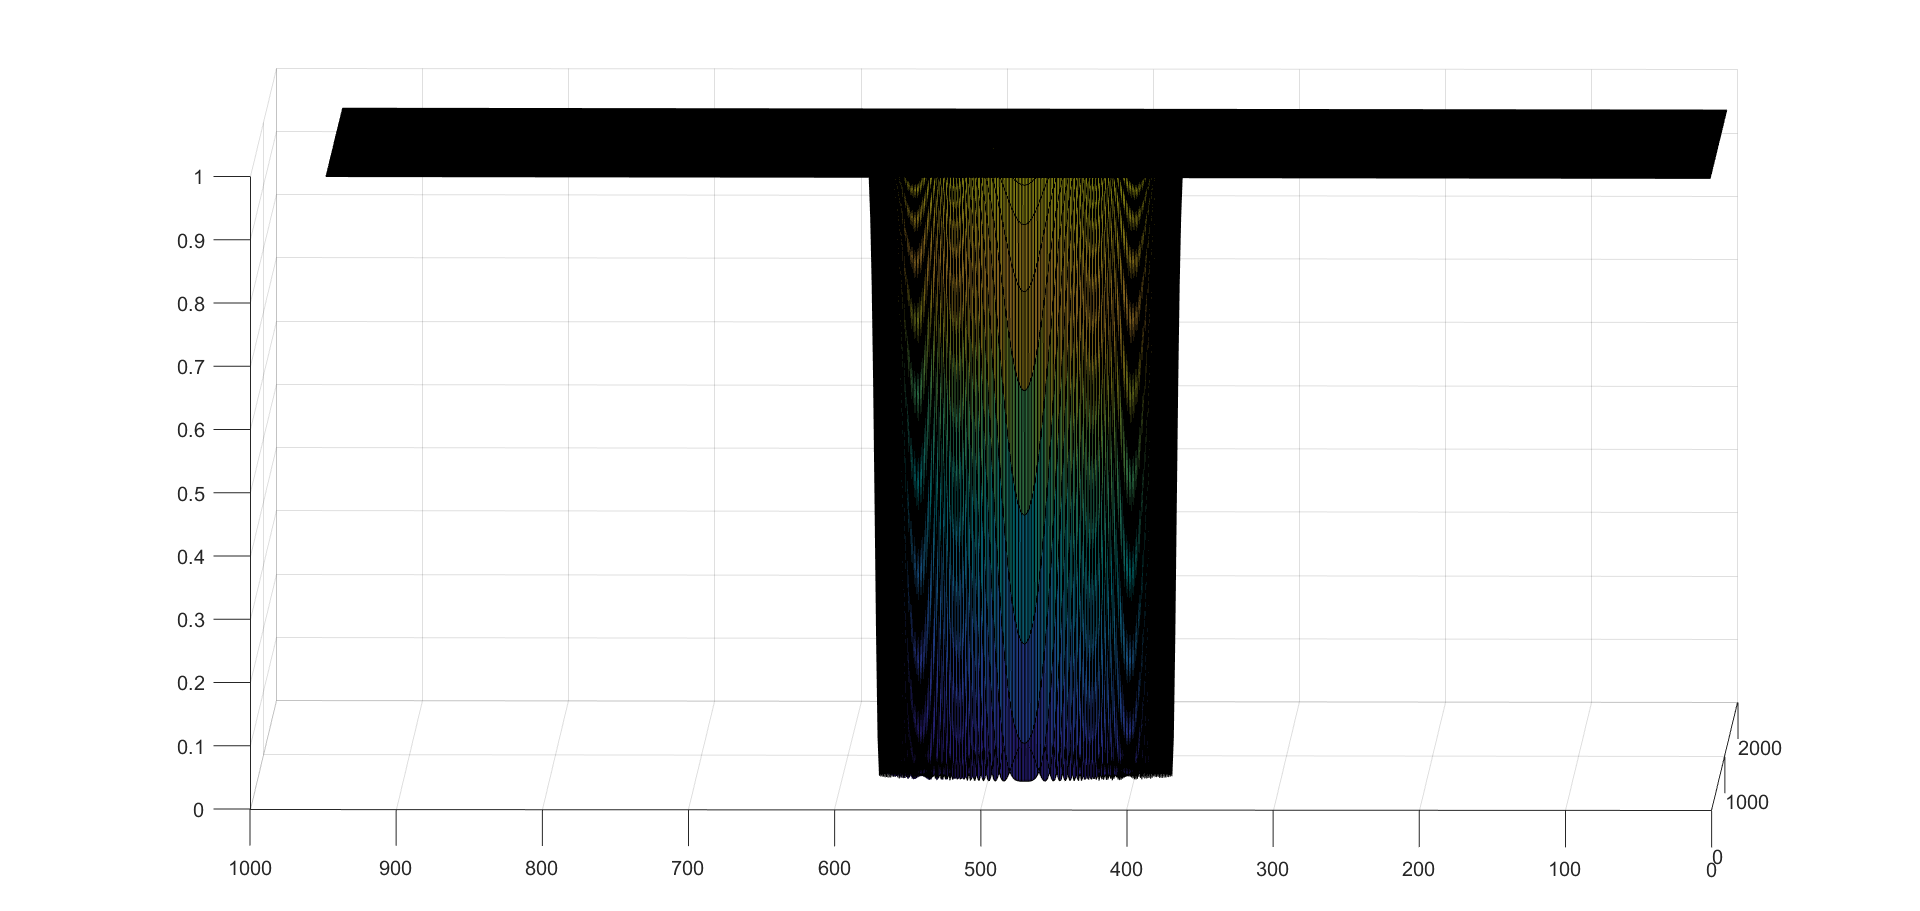
\includegraphics[width=\linewidth]{gaussian3d.png}
			\caption{gaussian.}
		\end{subfigure}
	\caption{cross-section of three filters.}
	\end{figure}
	In this case, there are no prominent differences between these three filters.From the cross-section image of these three filters, it suggests the width of the band is too narrow to differentiate the these three filters and what's more the order of butterworth filter is 4 which makes the function very steep which almost approximates ideal filter. So comments on the ability to recover original image should depend on the noise pattern and parameters of filters. In other words, it is necessary to design specific filter against specific noise.

\end{document}